% ============================================================
%  Sprawozdanie: Wyznaczanie stałej Plancka metodą optyczną
%  Fotonika – laboratorium, ZUT Szczecin
% ============================================================
\documentclass[a4paper,12pt]{article}

\usepackage[utf8]{inputenc}
\usepackage[T1]{fontenc}
\usepackage[polish]{babel}
\usepackage{geometry}
\geometry{a4paper, top=2.2cm, bottom=2.2cm, left=2.5cm, right=2.5cm}

\usepackage{amsmath,amssymb}
\usepackage{booktabs}
\usepackage{graphicx}
\usepackage{float}
\usepackage{caption}
\usepackage{subcaption}
\usepackage{multirow}
\usepackage{array}
\usepackage{xcolor}
\usepackage{hyperref}
\usepackage{siunitx}
\sisetup{output-decimal-marker={,}, locale=DE}
\usepackage{tikz}
\usetikzlibrary{circuits.ee.IEC, positioning}
\usepackage{parskip}
\setlength{\parskip}{4pt}

% ── tytuł dokumentu (dane w tabeli) ────────────────────────
\title{}
\date{}

\begin{document}

% ============================================================
%  TABELA NAGŁÓWKOWA
% ============================================================
\begin{table}[H]
\centering
\renewcommand{\arraystretch}{1.4}
\begin{tabular}{|p{4.2cm}|p{4.2cm}|p{4.2cm}|}
\hline
\multicolumn{3}{|p{12.9cm}|}{%
  \centering
  \textbf{Zachodniopomorski Uniwersytet Technologiczny w~Szczecinie}
  \newline
  Wydział Elektryczny\quad--\quad Katedra Telekomunikacji i~Fotoniki
  \newline
  \textbf{FOTONIKA -- Laboratorium}
  \newline
  \textbf{Ćwiczenie 06: Wyznaczanie stałej Plancka metodą optyczną (PLANCK)}
} \\
\hline
Kierunek: Elektronika i~Telekomunikacja &
  Semestr: IV & Nr zespołu: --- \\
\hline
\multicolumn{2}{|l|}{Skład zespołu: ---} &
  Prowadzący: --- \\
\hline
\multicolumn{2}{|l|}{Data wykonania ćwiczenia: 16 marca 2026} &
  Ocena: \phantom{XXXXX} \\
\hline
\end{tabular}
\end{table}

% ============================================================
\section*{1.\quad Cel ćwiczenia}
% ============================================================

Celem ćwiczenia jest wyznaczenie wartości stałej Plancka na podstawie pomiarów napięć
progowych charakterystyk prądowo-napięciowych diod LED w różnych kolorach oraz widm
emitowanego przez nie światła.

% ============================================================
\section*{2.\quad Wstęp teoretyczny}
% ============================================================

\textbf{Dioda elektroluminescencyjna (LED)} pracuje przy polaryzacji złącza PN w~kierunku
przewodzenia. W półprzewodnikach z~prostą przerwą energetyczną $E_G$ elektrony z~pasma
przewodnictwa rekombinują z~dziurami z~pasma walencyjnego, emitując fotony o~energii:
\begin{equation}
  h\nu = \frac{hc}{\lambda} \approx E_G,
  \label{eq:foton}
\end{equation}
gdzie $h$ – stała Plancka, $\nu$ – częstotliwość promieniowania, $\lambda$ – długość fali,
$c \approx \SI{3e8}{\metre\per\second}$ – prędkość światła w próżni.

Prąd diody opisuje zmodyfikowane równanie Shockleya:
\begin{equation}
  I = I_0 \exp\!\left(\frac{V - V_G}{V_T}\right),
  \label{eq:dioda}
\end{equation}
gdzie $V_G = E_G / q$ jest \textbf{napięciem progowym} odpowiadającym szerokości przerwy
energetycznej, $q = \SI{1.602e-19}{C}$ – ładunek elementarny, a~$V_T = k_BT/q \approx \SI{26}{mV}$
– napięcie termiczne. Napięcie $V_G$ wyznacza się graficznie jako punkt przecięcia stycznej do
liniowej części charakterystyki $I(U)$ z~osią napięcia (rys.~4 w~instrukcji).

Łącząc równania~(\ref{eq:foton}) i~(\ref{eq:dioda}) otrzymujemy zależność liniową między
napięciem progowym a częstotliwością emitowanego światła:
\begin{equation}
  V_G = \frac{h}{q}\cdot\nu = K\cdot\nu.
  \label{eq:planck_liniowy}
\end{equation}
Nachylenie prostej $K = h/q$ pozwala wyznaczyć stałą Plancka:
\begin{equation}
  h = K \cdot q.
  \label{eq:h}
\end{equation}
Wartość tablicowa: $h_\text{lit} = \SI{6.626e-34}{J.s}$.

% ============================================================
\section*{3.\quad Schemat układu pomiarowego}
% ============================================================

\begin{figure}[H]
\centering
\begin{tikzpicture}[circuit ee IEC, x=1.6cm, y=1.2cm,
    every info/.style={font=\small}]
  % zasilacz
  \draw (0,2) node[above, font=\small\bfseries] {Zasilacz}
              rectangle (1.4,0.4);
  \node[font=\small] at (0.7,1.2) {DC};
  % przewody z zasilacza
  \draw (1.4,1.6) -- (2.2,1.6);
  \draw (1.4,0.8) -- (2.2,0.8);
  % amperomierz
  \draw (2.2,1.6) -- (2.2,2.4) to[ammeter] (4.2,2.4) -- (4.2,1.6);
  % woltomierz
  \draw (2.2,0.8) -- (2.2,0.0) to[voltmeter] (4.2,0.0) -- (4.2,0.8);
  % dioda LED
  \draw (4.2,1.6) to[led, l=LED] (4.2,0.8);
  % zamknięcie obwodu
  \draw (2.2,1.6) -- (2.2,1.6);
  % spektrometr
  \draw[dashed, ->, thick] (4.8,1.2) -- (6.0,1.2)
      node[right, align=left, font=\small] {Światłowód\\spektrometru};
  \node[draw, rounded corners, align=center, font=\small\bfseries] at (7.6,1.2)
      {Spektrometr\\światłowodowy\\(laptop)};
\end{tikzpicture}
\caption{Schemat układu pomiarowego do wyznaczania stałej Plancka z~użyciem diod LED.}
\label{fig:schemat}
\end{figure}

% ============================================================
\section*{4.\quad Spis przyrządów pomiarowych}
% ============================================================

\begin{itemize}
  \item Zestaw diod LED: czerwona (R), zielona (G), niebieska (B) oraz żółta (Y)
        -- dioda żółta uległa uszkodzeniu podczas pomiarów i~nie zostały zebrane
        dla niej dane.
  \item Spektrometr światłowodowy z~oprogramowaniem \textit{Spectrometer} (Kvant 2018)
        wraz z~laptopem.
  \item Zasilacz napięcia stałego (regulowany).
  \item Dwa multimetry cyfrowe (woltomierz i~amperomierz).
\end{itemize}

% ============================================================
\section*{5.\quad Przebieg ćwiczenia}
% ============================================================

\begin{enumerate}
  \item Zestawiono układ jak na rys.~\ref{fig:schemat}. Do kolejnych gniazd podłączano
        każdą z~diod LED, pilnując nieprzekroczenia dopuszczalnych prądów:
        $I_\text{max} = \SI{30}{mA}$ dla diod R, Y, G i~$I_\text{max} = \SI{5}{mA}$
        dla diody B.
  \item Za pomocą spektrometru zarejestrowano widmo każdej świecącej diody.
        Odczytano środkową długość fali $\lambda_0$ (maximum krzywej dzwonowej) oraz
        połówkową szerokość widma $\Delta\lambda_{1/2}$ (\textit{FWHM}).
        Dane widmowe wyeksportowano do pliku \texttt{.txt}.
  \item Zmierzono charakterystyki statyczne $I(U)$ każdej diody (6 punktów pomiarowych
        na diodę), zaczynając od napięcia, przy którym dioda zaczyna wyraźnie się
        świecić. Na podstawie wykresu wyznaczono graficznie napięcie progowe $V_G$
        metodą stycznej.
  \item Sporządzono wykres $V_G(\nu)$ i~metodą regresji liniowej wyznaczono
        współczynnik~$K = h/q$, a~stąd stałą Plancka~$h$.
\end{enumerate}

% ============================================================
\section*{6.\quad Wyniki pomiarów i~opracowanie}
% ============================================================

\subsection*{6.1\quad Tabela~I – Parametry widm diod LED}

Centralna długość fali $\lambda_0$ i~szerokość połówkowa $\Delta\lambda_{1/2}$ zostały
wyznaczone z~danych spektrometrycznych (pliki \texttt{.txt}) skryptem
\texttt{analiza\_plancka.py}. Wyznaczono maximum wygładzonego widma
(filtr Savitzky-Golay) oraz punkty przecięcia z~połową jego wartości maksymalnej
(po odjęciu tła). Przyjęto dokładność pomiaru długości fali
$\Delta\lambda = \pm\SI{1}{nm}$ (zgodnie z~instrukcją).

Dioda żółta uległa przypadkowemu uszkodzeniu podczas zajęć, dlatego jej dane nie są
dostępne.

\begin{table}[H]
\centering
\caption{Parametry widm diod LED.}
\label{tab:widma}
\begin{tabular}{lccc}
\toprule
Dioda LED & $\lambda_0$ (nm) & $\Delta\lambda_{1/2}$ -- FWHM (nm) & Uwagi \\
\midrule
Czerwona (R) & 619 & 45 & \\
Żółta (Y)    & --- & --- & uszkodzona \\
Zielona (G)  & 563 & 47 & \\
Niebieska (B)& 471 & 27 & \\
\bottomrule
\end{tabular}
\end{table}

Zarejestrowane widma z~zaznaczoną centralną długością fali i~granicami FWHM przedstawia
rys.~\ref{fig:widma}.

\begin{figure}[H]
  \centering
  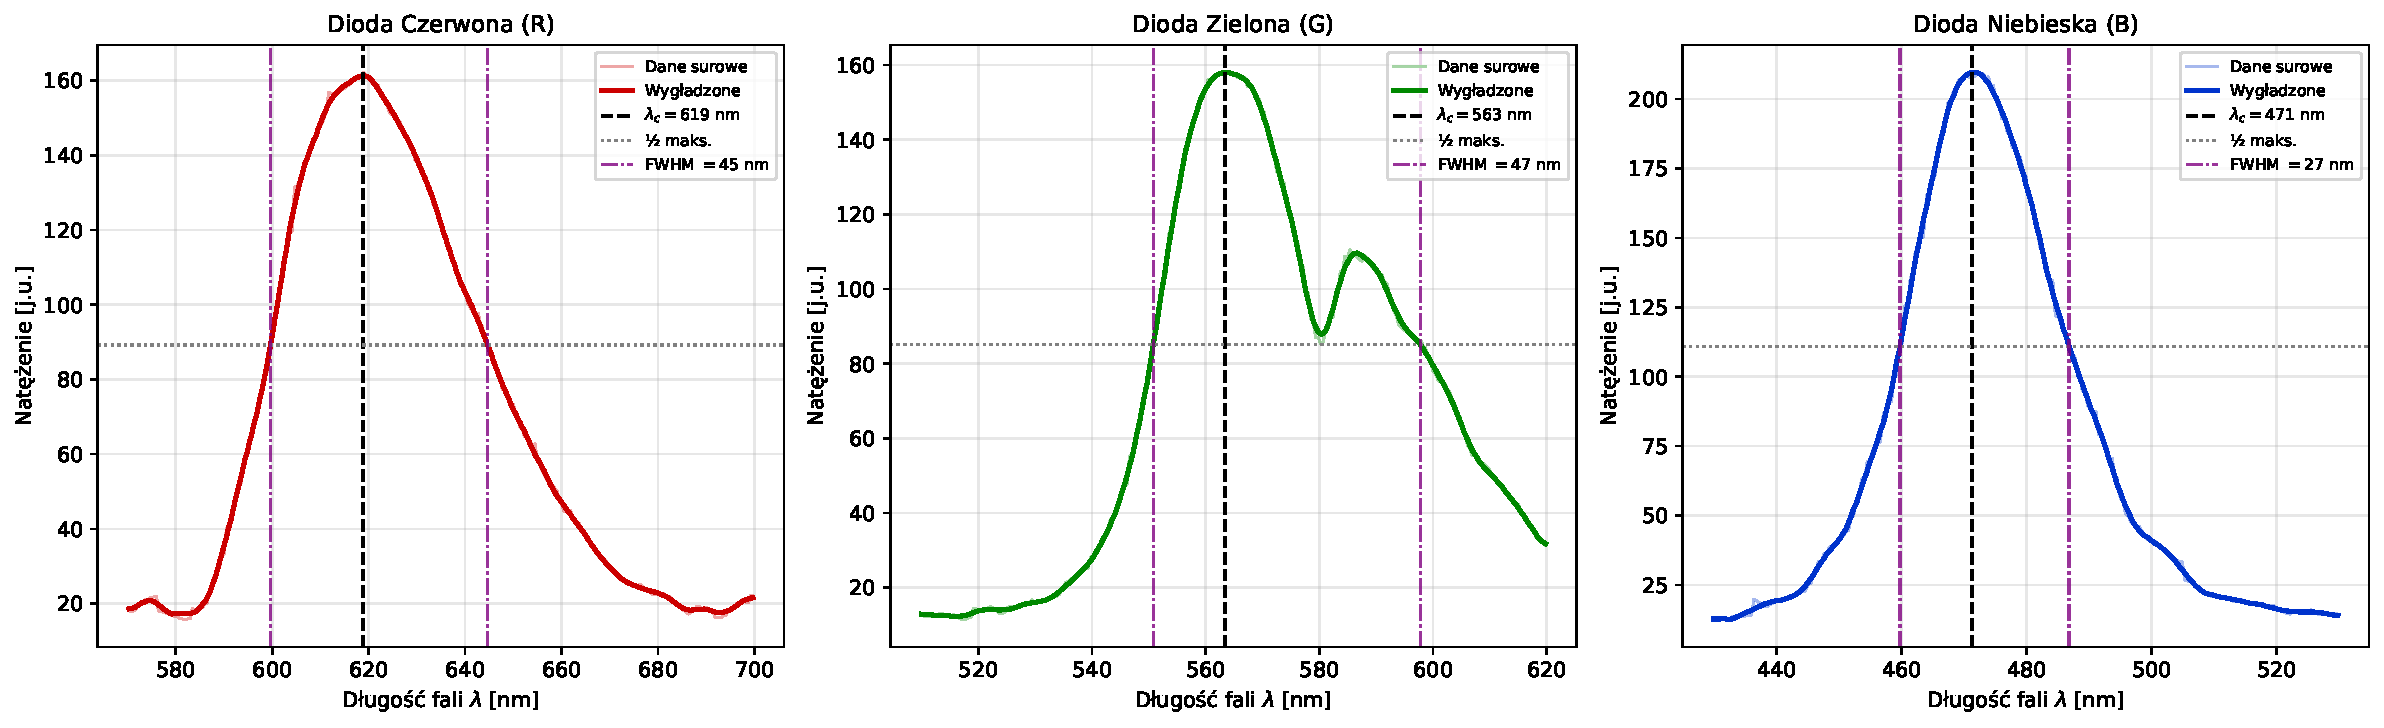
\includegraphics[width=\textwidth]{wykres_widm.pdf}
  \caption{Widma emisyjne diod LED. Linia przerywana – centralna długość fali $\lambda_0$;
           linie kropkowane – granice FWHM; pozioma linia – poziom półmaksimum.}
  \label{fig:widma}
\end{figure}

% ────────────────────────────────────────────────────────────
\subsection*{6.2\quad Tabela~II – Charakterystyki $I(U)$ diod LED}

\begin{table}[H]
\centering
\caption{Zmierzone wartości napięcia $U$ [V] i~natężenia prądu $I$ [mA]
         dla charakterystyk statycznych diod LED.}
\label{tab:IU}
\renewcommand{\arraystretch}{1.15}
\begin{tabular}{c*{6}{S[table-format=1.2]S[table-format=2.2]}}
\toprule
 & \multicolumn{2}{c}{\textbf{Czerwona}} &
   \multicolumn{2}{c}{\textbf{Żółta}} &
   \multicolumn{2}{c}{\textbf{Zielona}} &
   \multicolumn{2}{c}{\textbf{Niebieska}} \\
\cmidrule(lr){2-3}\cmidrule(lr){4-5}\cmidrule(lr){6-7}\cmidrule(lr){8-9}
Lp. & {$U$ (V)} & {$I$ (mA)} & {$U$ (V)} & {$I$ (mA)}
    & {$U$ (V)} & {$I$ (mA)} & {$U$ (V)} & {$I$ (mA)} \\
\midrule
1 & 1.67 & 1  & {---} & {---} & 1.80 & 1    & 2.60 & 0.10 \\
2 & 1.76 & 4  & {---} & {---} & 1.86 & 3    & 2.68 & 0.20 \\
3 & 1.83 & 8  & {---} & {---} & 1.93 & 6    & 2.87 & 0.75 \\
4 & 1.91 & 15 & {---} & {---} & 2.00 & 12   & 3.00 & 1.50 \\
5 & 1.97 & 20 & {---} & {---} & 2.16 & 24   & 3.19 & 3.00 \\
6 & 2.02 & 25 & {---} & {---} & 2.22 & 30   & 3.27 & 4.00 \\
\bottomrule
\end{tabular}
\end{table}

Charakterystyki $I(U)$ z~zaznaczonymi napięciami progowymi $V_G$ wyznaczonymi metodą
stycznej przedstawia rys.~\ref{fig:IU}.

\begin{figure}[H]
  \centering
  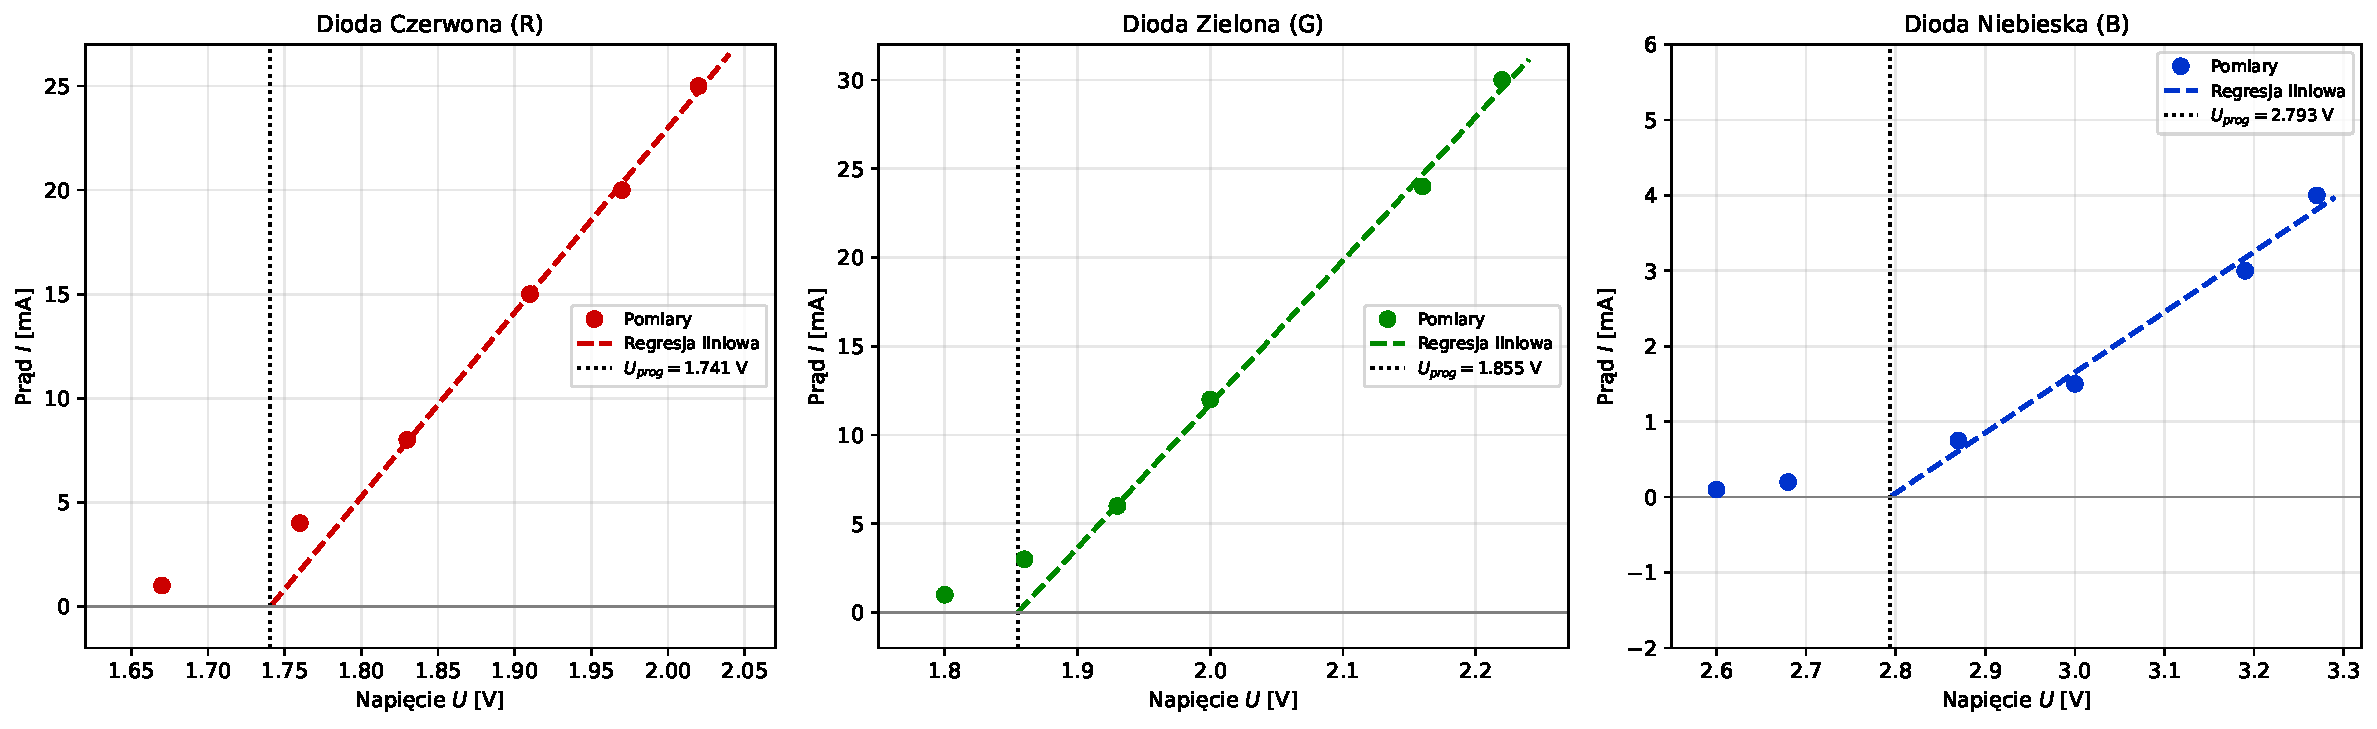
\includegraphics[width=\textwidth]{wykres_IU.pdf}
  \caption{Charakterystyki prądowo-napięciowe $I(U)$ diod LED. Linia przerywana –
           regresja liniowa na ostatnich czterech punktach; linia kropkowana –
           napięcie progowe $V_G$.}
  \label{fig:IU}
\end{figure}

Napięcie progowe wyznaczono jako punkt przecięcia prostej regresji liniowej (dopasowanej
do liniowej części charakterystyki, tj.~czterech ostatnich punktów pomiarowych) z~osią
napięcia. Niepewność $\Delta V_G \approx \SI{0.05}{V}$ oszacowano na podstawie rozrzutu
danych wokół prostej dopasowania.

% ────────────────────────────────────────────────────────────
\subsection*{6.3\quad Tabela~III – Zestawienie wyników pośrednich}

\begin{table}[H]
\centering
\caption{Napięcia progowe, częstotliwości i~pośrednie wartości $K = h/q$
         dla diod LED.}
\label{tab:III}
\renewcommand{\arraystretch}{1.25}
\setlength{\tabcolsep}{5pt}
\begin{tabular}{lS[table-format=1.3]S[table-format=1.2]S[table-format=3.0]S[table-format=1.0]
               S[table-format=1.3]S[table-format=1.3]S[table-format=1.3]}
\toprule
Dioda &
  {$V_G$} & {$\Delta V_G$} &
  {$\lambda_0$} & {$\Delta\lambda_0$} &
  {$\nu$} &
  {$K\!=\!V_G/\nu$} &
  {$h_i$} \\
  & {(V)} & {(V)} & {(nm)} & {(nm)} & {($10^{14}$\,Hz)}
  & {($10^{-15}$\,V\,s)} & {($10^{-34}$\,J\,s)} \\
\midrule
Czerwona & 1.741 & 0.05 & 619 & 1 & 4.844 & 3.594 & 5.758 \\
Żółta    & {---} & {---}& {---}& {---}& {---} & {---} & {---} \\
Zielona  & 1.855 & 0.05 & 563 & 1 & 5.321 & 3.486 & 5.585 \\
Niebieska& 2.793 & 0.05 & 471 & 1 & 6.361 & 4.391 & 7.034 \\
\bottomrule
\end{tabular}
\end{table}

\noindent\textbf{Uwaga:} Kolumna $h_i$ zawiera wartości \emph{pomocnicze} do identyfikacji
danych na wykresie. Wynikiem doświadczenia jest \textbf{jedna} wartość $h$ wyznaczona
z~regresji liniowej (poniżej).

% ────────────────────────────────────────────────────────────
\subsection*{6.4\quad Wykres $V_G(\nu)$ i~wyznaczenie stałej Plancka}

Zgodnie z równaniem~(\ref{eq:planck_liniowy}), wykres $V_G$ w funkcji $\nu = c/\lambda_0$
powinien być linią prostą przechodzącą przez początek układu współrzędnych
o~nachyleniu $K = h/q$. Wykonano regresję liniową przez początek układu (model fizyczny
wymaga wyrazuz wolnego równego zero):
\begin{equation}
  K = \frac{\sum_i \nu_i V_{G,i}}{\sum_i \nu_i^2}.
\end{equation}

\begin{figure}[H]
  \centering
  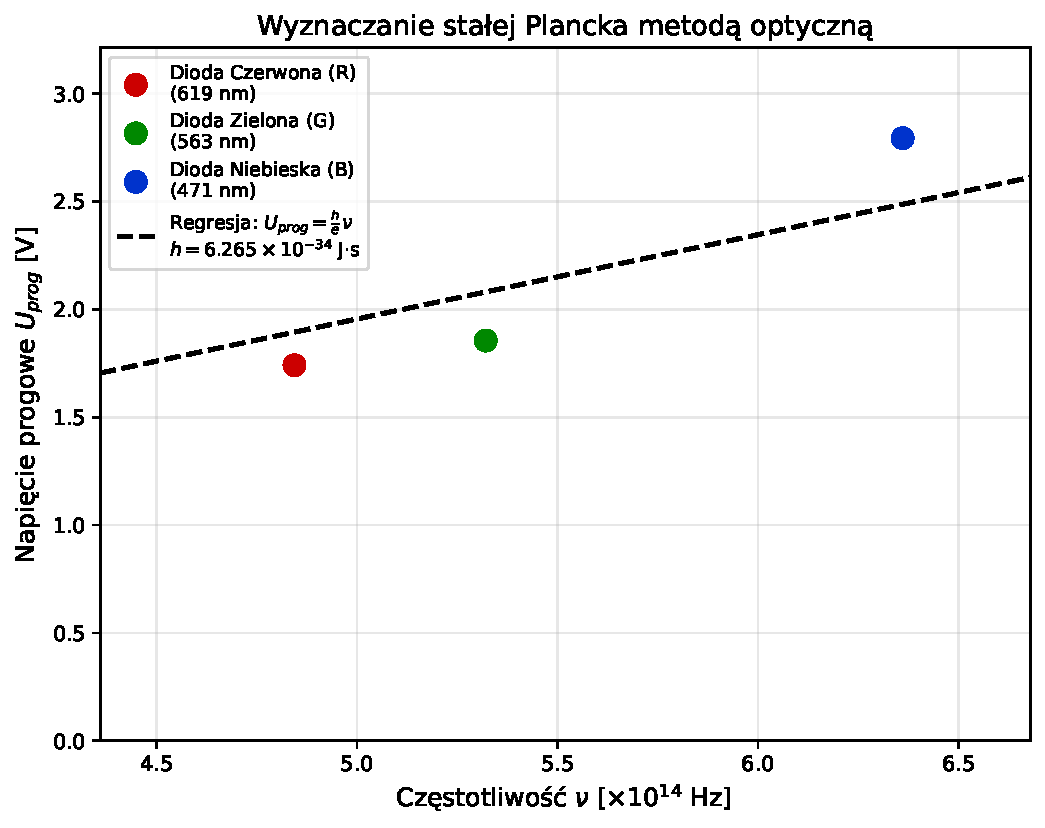
\includegraphics[width=0.75\textwidth]{wykres_Plancka.pdf}
  \caption{Wykres $V_G(\nu)$ dla trzech diod LED wraz z~regresją liniową
           $V_G = K\cdot\nu$. Wartość stałej Plancka odczytana ze współczynnika
           nachylenia prostej.}
  \label{fig:planck}
\end{figure}

Uzyskano:
\begin{equation*}
  K = \frac{h}{q} = \SI{3{,}910e-15}{V.s}.
\end{equation*}

Stała Plancka:
\begin{equation*}
  h = K \cdot q = \SI{3{,}910e-15}{V.s} \times \SI{1{,}602e-19}{C}
    = \SI{6{,}264e-34}{J.s}.
\end{equation*}

% ────────────────────────────────────────────────────────────
\subsection*{6.5\quad Analiza niepewności}

Wynik doświadczenia wyrażamy jako $h = K \cdot q$, gdzie $q$ traktujemy jako stałą dokładną.
Niepewność stałej Plancka pochodzi od niepewności $\Delta K$.

\subsubsection*{Niepewność statystyczna $\Delta K_\text{stat}$ (z~reszt regresji)}

Dla regresji przez początek układu (jeden parametr wolny, $n=3$ punkty, $df = n-1 = 2$):
\begin{equation}
  \Delta K_\text{stat} = \frac{s}{\sqrt{\sum_i \nu_i^2}}, \qquad
  s = \sqrt{\frac{\sum_i (V_{G,i} - K\nu_i)^2}{n-1}}.
\end{equation}
Reszty wynoszą: $e_\text{R} = -0{,}153$\,V, $e_\text{G} = -0{,}226$\,V, $e_\text{B} = +0{,}306$\,V.
\begin{align*}
  s &= \sqrt{\frac{(-0{,}153)^2 + (-0{,}226)^2 + (0{,}306)^2}{2}}
     = \SI{0{,}2897}{V}, \\[4pt]
  \Delta K_\text{stat} &= \frac{0{,}2897}{\sqrt{5{,}2034 \times 10^{29}}}
     = \SI{4{,}016e-16}{V.s}.
\end{align*}

\subsubsection*{Niepewność pomiarowa $\Delta K_\text{meas}$ (z~propagacji $\Delta V_G$ i~$\Delta\lambda_0$)}

Dla wzoru $K = \frac{\sum_i \nu_i V_{G,i}}{\sum_i \nu_j^2}$ stosujemy prawo przenoszenia błędów:
\begin{equation}
  \Delta K_\text{meas} = \sqrt{
    \sum_i \left(\frac{\partial K}{\partial V_{G,i}}\right)^2 (\Delta V_{G,i})^2 +
    \sum_i \left(\frac{\partial K}{\partial \nu_i}\right)^2  (\Delta\nu_i)^2},
\end{equation}
gdzie $\Delta\nu_i = \frac{c}{\lambda_i^2}\,\Delta\lambda_i$.
Obliczenia numeryczne dają: $\Delta K_\text{meas} = \SI{5{,}22e-17}{V.s}$.

\subsubsection*{Łączna niepewność standardowa}

\begin{equation}
  \Delta K = \sqrt{(\Delta K_\text{stat})^2 + (\Delta K_\text{meas})^2}
           = \SI{3{,}061e-16}{V.s}.
\end{equation}

\subsubsection*{Niepewność rozszerzona ($k = 2$, poziom ufności $\approx 95\%$)}

\begin{align}
  \Delta h &= \Delta K \cdot q = \SI{3{,}061e-16}{V.s} \times \SI{1{,}602e-19}{C}
             = \SI{4{,}904e-35}{J.s}, \notag\\[4pt]
  \Delta h_\text{rozsz} &= k \cdot \Delta h = 2 \times \SI{4{,}904e-35}{J.s}
             = \SI{9{,}808e-35}{J.s}.
\end{align}

\subsubsection*{Wynik końcowy}

\begin{equation}
  \boxed{h = (6{,}264 \pm 0{,}981) \times 10^{-34}\ \text{J\,s}}
  \qquad (k=2,\ \text{poziom ufności} \approx 95\%)
\end{equation}

Wartość tablicowa $h_\text{lit} = \SI{6{,}626e-34}{J.s}$ mieści się w~przedziale
niepewności wyznaczonego wyniku
($5{,}283 \times 10^{-34}\ \text{J\,s} \leq h_\text{lit} \leq 7{,}245 \times 10^{-34}\ \text{J\,s}$),
co potwierdza poprawność doświadczenia.

Błąd względny wyniku:
\begin{equation*}
  \delta h = \frac{|h - h_\text{lit}|}{h_\text{lit}} \times 100\%
           = \frac{|6{,}264 - 6{,}626|}{6{,}626} \times 100\% \approx 5{,}5\%.
\end{equation*}

% ============================================================
\section*{7.\quad Wnioski}
% ============================================================

\begin{enumerate}
  \item Wyznaczona wartość stałej Plancka
        $h = (6{,}264 \pm 0{,}981) \times 10^{-34}$\,J\,s jest zgodna z~wartością
        tablicową $h_\text{lit} = 6{,}626 \times 10^{-34}$\,J\,s; wartość literaturowa
        leży wewnątrz przedziału niepewności, a~błąd względny wynosi ok.\ $5{,}5\%$.

  \item Centralne długości fal wyznaczone ze spektrometru wynoszą:
        $\lambda_0^\text{R} = \SI{619}{nm}$,
        $\lambda_0^\text{G} = \SI{563}{nm}$,
        $\lambda_0^\text{B} = \SI{471}{nm}$,
        co odpowiada barwom emitowanego światła i~spodziewanym wartościom dla
        stosowanych materiałów półprzewodnikowych (odpowiednio GaAsP, InGaN/GaP
        i~InGaN).

  \item Połówkowe szerokości widm (FWHM) wynoszą 27--47\,nm, co jest typowe dla
        diod LED i~wynika ze skończonej temperatury złącza oraz rozkładu energii
        nośników.

  \item \textbf{Brak danych dla diody żółtej} (przypadkowe uszkodzenie) zmniejszył
        liczbę punktów na wykresie $V_G(\nu)$ z~czterech do trzech, co zwiększyło
        niepewność regresji. Gdyby dysponować czterema punktami, niepewność byłaby
        mniejsza, a~wynik dokładniejszy.

  \item Głównym źródłem niepewności jest rozrzut reszt regresji ($\Delta K_\text{stat}$),
        który dominuje nad niepewnością z~propagacji błędów pomiarowych
        ($\Delta K_\text{meas}$). Przyczyną rozrzutu może być niedokładność graficznego
        wyznaczania $V_G$ metodą stycznej oraz fakt, że model $V_G = (h/q)\nu$
        jest przybliżeniem (w rzeczywistości istnieją dodatkowe efekty, np.\ różnica
        funkcji wyjścia kontaktów metalu i~wpływ temperatury).

  \item Metoda optyczna wyznaczania stałej Plancka jest stosunkowo prosta i~daje
        wyniki bliskie wartości tablicowej przy użyciu tanich, łatwo dostępnych
        elementów optoelektronicznych.
\end{enumerate}

\end{document}
